\chapter{Results and Discussion}

\section{Overview of the evaluation}

This chapter evaluates whether dictionary-assisted normalization and hybrid retrieval improve responses to code-switched local government service inquiries. It addresses the three research objectives stated in Chapter 1: implementing an approach that captures charter identifiers and conversational intent, comparing the proposed architecture with retrieval baselines, and evaluating answer relevance and factual faithfulness through automated and human assessment. The results support different conclusions at different stages of the pipeline. Hybrid configurations retrieved relevant material more effectively than the raw-query BM25 baseline in the original evaluable subset. The expert audit, however, did not establish statistically significant differences in normalization fidelity or final answer quality among the compared configurations.


The automated evaluation used 70 held-out scenario groups, each expressed in English, Taglish and Bislish. All three architectures processed the resulting 210 queries, producing 630 archived outcomes. A separate development set contained 30 groups and 90 queries. Development data were used for selection of retrieval settings; the held-out outputs were retained without rewriting unsuccessful answers. The human audit covered the fixed category-balanced subset of 20 groups, four each from the Business Bureau, City Treasurer's Office, Office of the City Building Official, Bureau of Fire Protection, and City Planning and Development Office.


Configuration A used the original query with BM25 retrieval. Configuration B used query-specific municipal dictionary injection, constrained normalization and hybrid retrieval. Configuration C disabled query-specific injection while retaining the remaining B pipeline. All configurations used the registered Mistral generator and answer prompt. Configuration C retained shared static lexical guidance, so the B-C comparison isolates the incremental contribution of query-specific injection within that shared guidance rather than every possible form of dictionary knowledge.


The automated results are judgments and retrieval measurements, not proof that all source facts or answers are correct. The human scores are analyzed as independently assigned expert ratings on the researcher's explicit confirmation. Earlier assessment files carried conflicting preparation metadata; the originals, correction record and unchanged numerical scores are retained. The analysis did not independently observe the scoring sessions, and the reliability coefficients do not establish the provenance of collection.


\section{Implementation of the evaluated architecture}

The evaluated corpus contains 1,082 chunks derived from 358 source pages. Preprocessing retained source document and page identifiers and used actual-token windows of 120 tokens with 20-token overlap, with shorter terminal windows where necessary. Table-representation repairs were preserved separately from earlier extraction artifacts. Retrieval operated at chunk level, rather than using section-level repair pilots. These decisions support traceability from a generated response to the passages that were available to the model.


The registered configuration selected K=3 and fusion weights of 0.75 for BM25, 0.25 for dense retrieval and 0 for the dictionary retrieval boost. The zero retrieval-boost weight does not remove dictionary injection before normalization in Configuration B. It indicates that the selected candidate did not assign an additional contribution to the dictionary component of the retrieval score. Generation used temperature 0, top-p 0, an 8,192-token context setting and a maximum prediction setting of 1,536 tokens; normalization used a maximum prediction setting of 150. These settings were recorded for reproducibility, without treating deterministic settings as a guarantee of identical results across every runtime or hardware environment.


The conceptual sequence remains dictionary-assisted normalization, chunk-level retrieval, grounded answer generation and offline evaluation. RAGAS was used after generation; it was not an online judge that repeatedly repaired or regenerated answers. The implementation therefore addresses Objective 1 at the system-construction level. Whether these components improved the measured outcomes is considered separately below.


\section{Execution coverage and unsuccessful outcomes}

Table 4.1 reports all archived generation dispositions. Clarification and incomplete generation are explicit outcomes rather than silently removed examples. The term answered identifies the recorded generation status and does not certify factual accuracy.


{\small\begin{longtable}{@{}p{1.172in}p{1.172in}p{1.172in}p{1.172in}p{1.172in}@{}}\toprule

Configuration & Planned queries & Answered & Clarification required & Incomplete generation \\ \midrule\endhead

A & 210 & 209 & 0 & 1 \\

B & 210 & 204 & 5 & 1 \\

C & 210 & 203 & 5 & 2 \\

\bottomrule\end{longtable}}

Table 4.1. Final generation coverage. Source: current completion assessment and archived A/B/C outcomes.


All 630 planned outcomes are present and scoring attempts are complete, but not every metric is observed for every query. A missing judge score is not automatically a zero or a successful judgment. Matched comparisons use the intersection of queries with an observed value for the metric in all three configurations. Consequently, denominators vary across the automated measures and must accompany the reported means.


\section{Retrieval label versions and automated results}

The source-ID crosswalk registered in the execution manifest transferred 77 of 87 legacy source spans and yielded complete retrieval labels for 59 of 70 groups, or 177 queries. A later crosswalk contains ten additional table/source-page reconciliations, extending label coverage to all 210 queries. The later file has a different hash from the crosswalk recorded before inference. Some current summary fields show 210-query coverage while older narrative text still describes 177 queries.


This chapter separates the two label versions. Table 4.2 presents retrieval measurements on the original 177-query complete-label subset and matched RAGAS results on their own observed subsets. The retrieval means were recomputed from per-query values restricted to the original crosswalk's eligible queries and reproduce the historical complete-case results. Table 4.3 shows the current 210-query reconciled retrieval export separately. This drafting step did not independently recertify the ten later source mappings; their recorded source-page descriptions and hashes remain in the evidence archive. The second table is not presented as if its labels were all registered before inference.


{\small\begin{longtable}{@{}p{1.172in}p{1.172in}p{1.172in}p{1.172in}p{1.172in}@{}}\toprule

Metric & Matched queries & A & B & C \\ \midrule\endhead

Hit@3 & 177 & 0.5593 & 0.6667 & 0.6667 \\

MRR@3 & 177 & 0.3588 & 0.5565 & 0.5508 \\

Faithfulness & 188 & 0.7481 & 0.7636 & 0.7594 \\

Context precision & 202 & 0.8486 & 0.9191 & 0.9171 \\

Context recall & 202 & 0.8437 & 0.8415 & 0.8448 \\

Answer relevancy & 202 & 0.5794 & 0.5827 & 0.5956 \\

\bottomrule\end{longtable}}

Table 4.2. Matched automated results. Hit@3 and MRR@3 use the original complete-label subset. RAGAS denominators are metric-specific shared complete cases. Values are descriptive means.


\begin{center}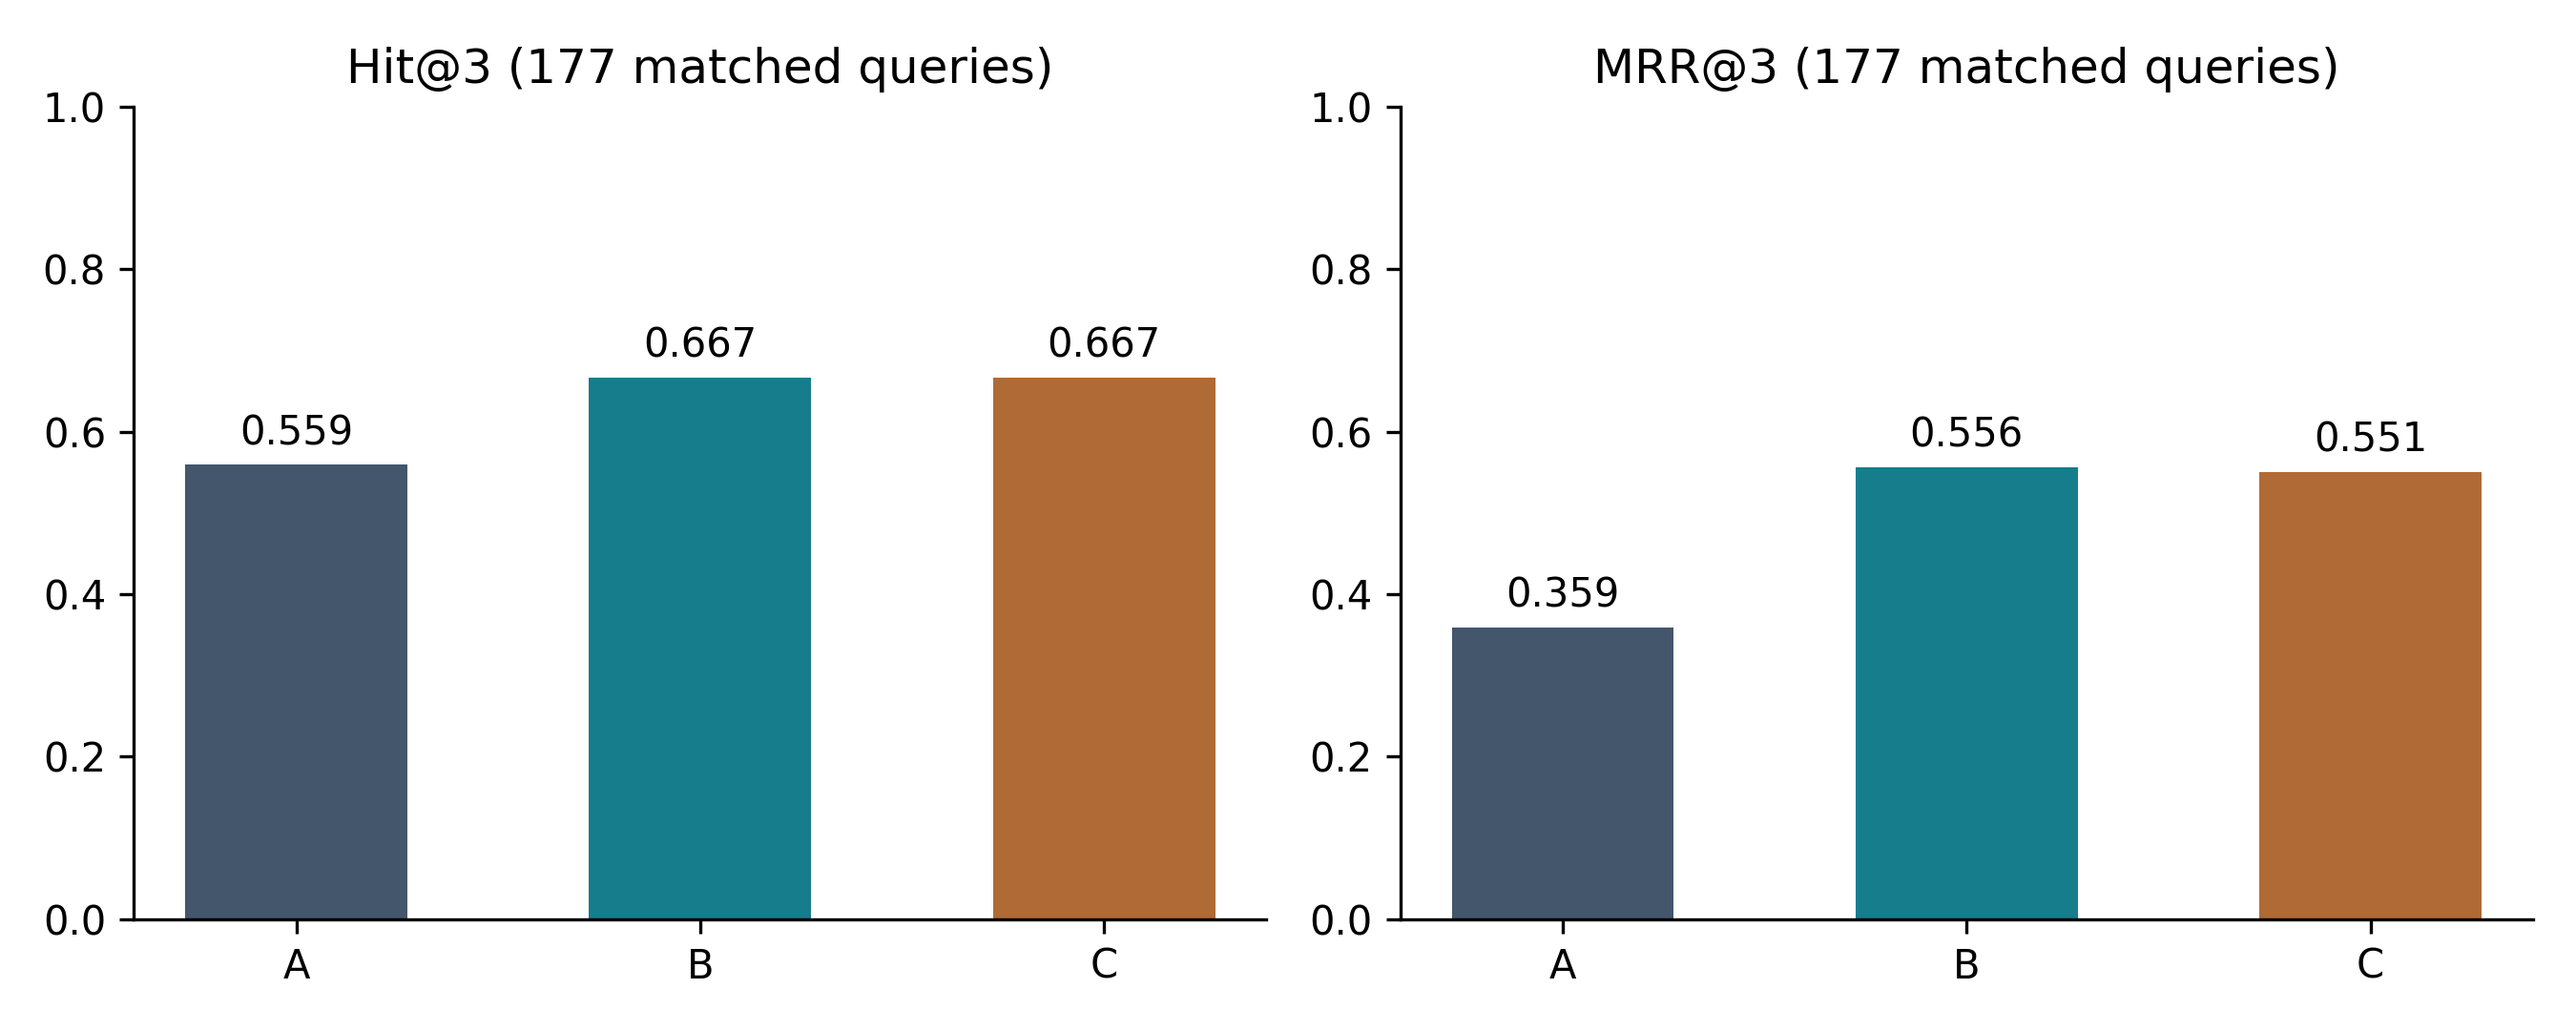
\includegraphics[width=\textwidth]{../figures/figure_4_1_retrieval.png}\end{center}

Figure 4.1. Retrieval performance on 177 queries with complete original span-transfer labels. Bar heights are descriptive; no significance test is implied by this figure.


On the original complete-label subset, B increased Hit@3 from 0.5593 to 0.6667 relative to A, a difference of approximately 10.73 percentage points. B also increased MRR@3 from 0.3588 to 0.5565. C had the same Hit@3 as B and a slightly lower MRR@3 of 0.5508. These observations are consistent with a benefit from the normalization-plus-hybrid pipeline over raw-query lexical retrieval, but they do not attribute the entire gain to dictionary injection. B and C share most of the pipeline and their retrieval results are close.


{\small\begin{longtable}{@{}p{1.172in}p{1.172in}p{1.172in}p{1.172in}p{1.172in}@{}}\toprule

Metric & Matched queries & A & B & C \\ \midrule\endhead

Hit@3 & 210 & 0.5762 & 0.6810 & 0.6857 \\

MRR@3 & 210 & 0.3659 & 0.5714 & 0.5659 \\

\bottomrule\end{longtable}}

Table 4.3. Current retrieval export after the additional ten source-span reconciliations. These 210-query measurements are disclosed as a later label version, separate from Table 4.2.


For automated answer evaluation, B's matched faithfulness mean was 0.7636, compared with 0.7481 for A and 0.7594 for C. B's context precision was 0.9191, compared with 0.8486 and 0.9171. Differences in context recall and answer relevancy did not consistently favor B: C had the largest means for those two measures. The results therefore do not support a blanket statement that B was best on every evaluation criterion.


The local Mistral evaluator has documented semantic and formatting failures. Its role as both generator family and judge family is another limitation. The reported RAGAS means summarize available automated judgments; they should be interpreted alongside missing-score counts, retrieved evidence and the human audit rather than as independently certified factual correctness. No new judge run was used to improve these numbers during manuscript drafting.


\section{Human audit allocation and normalization results}

The adviser-directed amendment introduced two human modules. Module 1 compared the B and C normalized queries for the 20 Taglish and 20 Bislish inputs in the audit subset. Each of three experts scored 80 outputs using the approved five-point statement about preservation of meaning, intent and explicit details, yielding 240 ratings. Module 2 compared the A, B and C final answers for all 60 queries, yielding 180 answer reviews per expert and 540 reviews overall. Two separate four-point dimensions produced 1,080 Module 2 scores. Together the modules contain 780 output-review records and 1,320 dimension scores.


All six supplied assessment files matched the issued packet identities, output IDs, question and output text, presentation order, expected score ranges and corresponding CSV values. No scores were changed or imputed during consolidation. Individual records are retained in a private analysis archive. The different scales were kept separate throughout analysis.


{\small\begin{longtable}{@{}p{1.172in}p{1.172in}p{1.172in}p{1.172in}p{1.172in}@{}}\toprule

Module / dimension & Config & Scores & Mean & Median \\ \midrule\endhead

M1 fidelity & B & 120 & 3.7583 & 4 \\

M1 fidelity & C & 120 & 3.7667 & 4 \\

M2 relevance & A & 180 & 2.3222 & 2 \\

M2 relevance & B & 180 & 2.2833 & 2 \\

M2 relevance & C & 180 & 2.2778 & 2 \\

M2 faithfulness & A & 180 & 2.7167 & 3 \\

M2 faithfulness & B & 180 & 2.7278 & 3 \\

M2 faithfulness & C & 180 & 2.6222 & 3 \\

\bottomrule\end{longtable}}

Table 4.4. Expert score distributions summarized by configuration. Means use numeric ordinal coding and are accompanied by medians; full score frequencies and language breakdowns are available in the accompanying CSV.


\begin{center}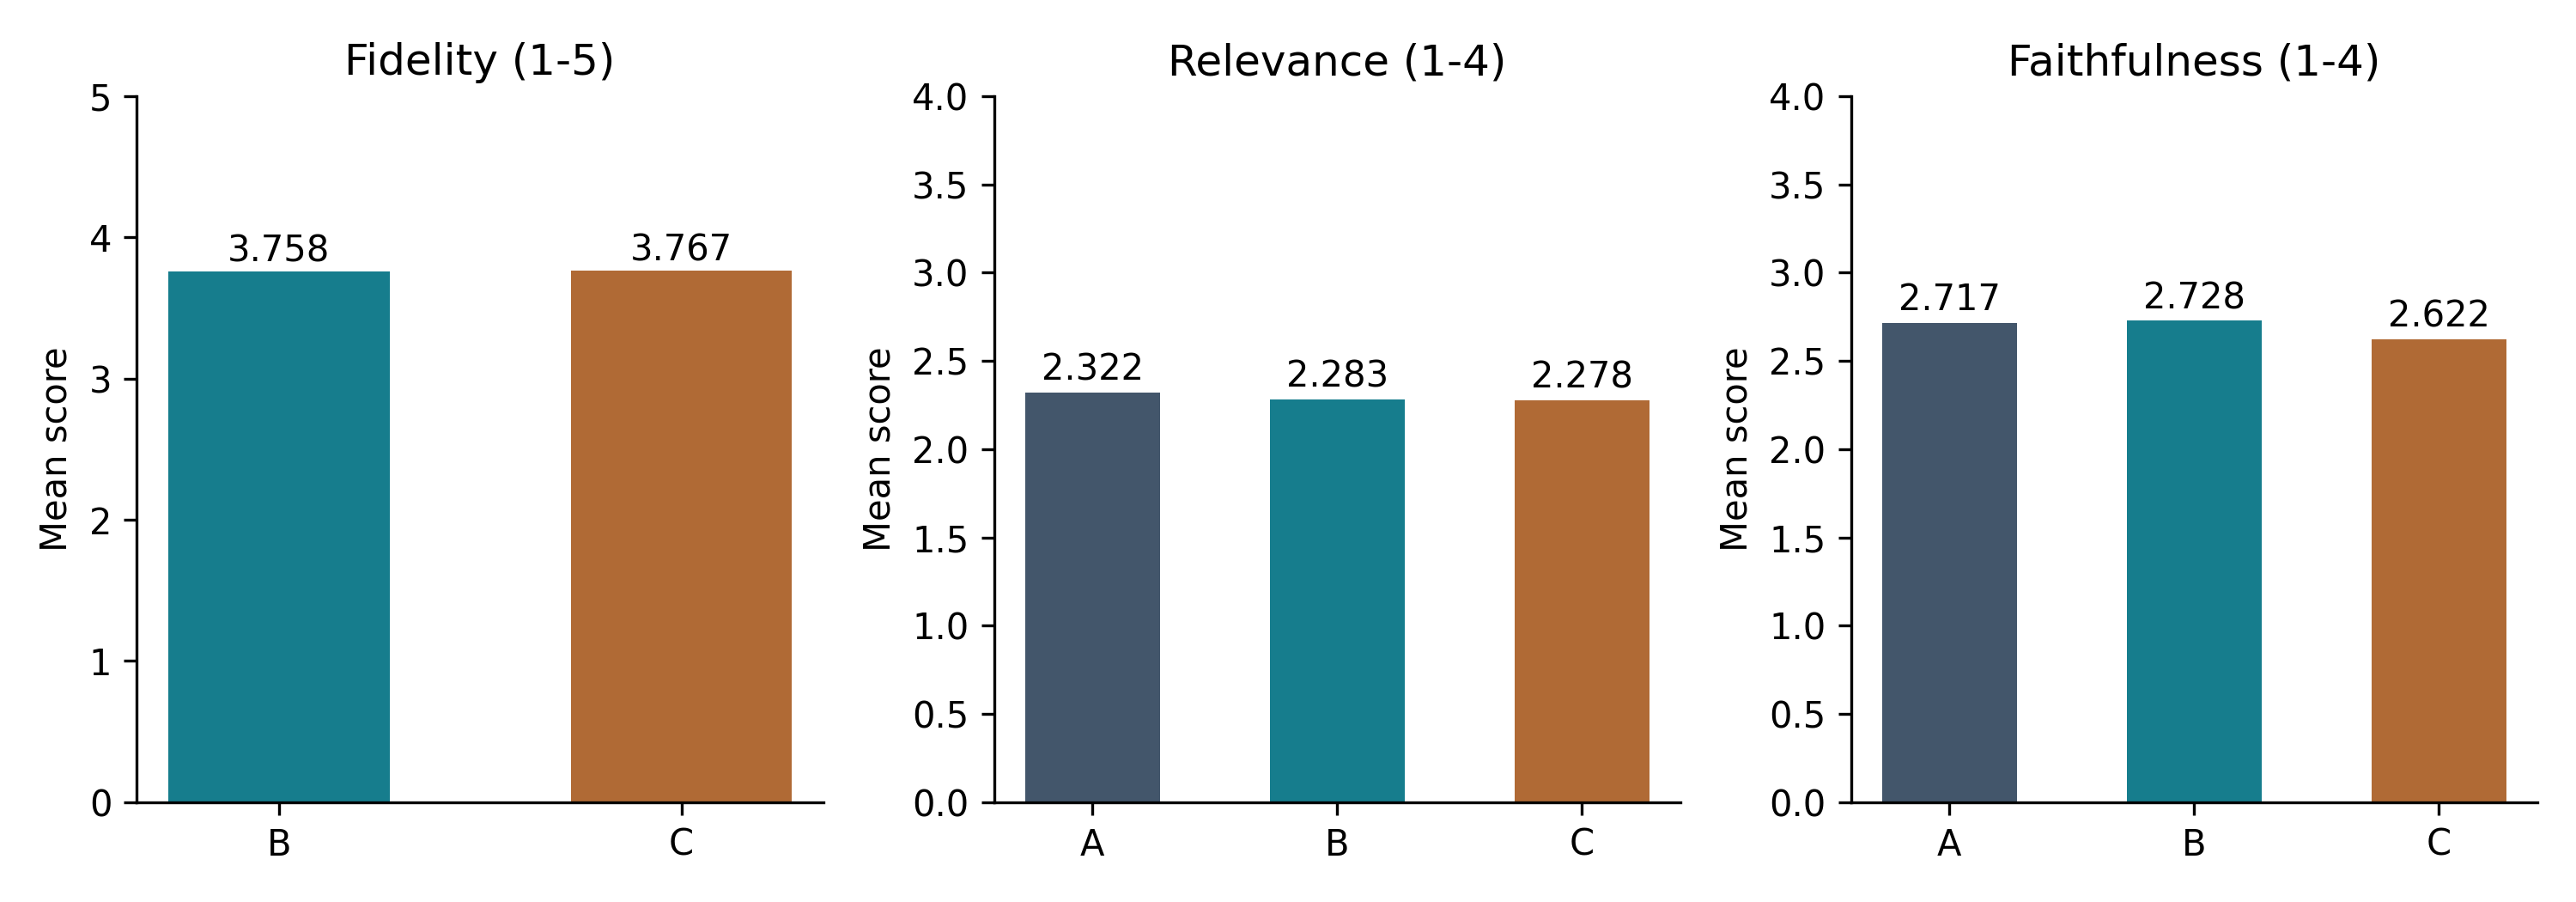
\includegraphics[width=\textwidth]{../figures/figure_4_2_human_means.png}\end{center}

Figure 4.2. Descriptive expert means. Normalization uses a five-point agreement scale; answer relevance and faithfulness use four-point scales. The panels must not be combined into a single cross-module score.


B and C normalization means were 3.7583 and 3.7667, respectively. Both medians were 4. These values indicate that many outputs were judged to preserve the original inquiry, while the distributions still include lower fidelity judgments. The very small aggregate B-C difference does not establish an additional fidelity benefit from query-specific dictionary injection on this sample. Language-specific summaries are descriptive diagnostics and are not additional unadjusted significance claims.


The frequency distribution in Table 4.5 gives the ordinal means a clearer interpretation. In Module 1, 74 of 120 ratings (61.7\%) were 4 or 5 for each configuration. These are ratings of 40 outputs by three raters per configuration, not 120 independent citizen inquiries. The remaining ratings include neutral and disagreement responses, so neither configuration preserved every inquiry reliably.


{\small\begin{longtable}{@{}p{0.672in}p{0.672in}p{0.672in}p{0.672in}p{0.672in}p{0.672in}p{0.672in}p{0.672in}@{}}\toprule

Dimension & Config & N & 1 & 2 & 3 & 4 & 5 \\ \midrule\endhead

M1 fidelity & B & 120 & 7 & 20 & 19 & 23 & 51 \\

M1 fidelity & C & 120 & 7 & 24 & 15 & 18 & 56 \\

M2 relevance & A & 180 & 52 & 56 & 34 & 38 & - \\

M2 relevance & B & 180 & 59 & 51 & 30 & 40 & - \\

M2 relevance & C & 180 & 59 & 51 & 31 & 39 & - \\

M2 faithfulness & A & 180 & 33 & 48 & 36 & 63 & - \\

M2 faithfulness & B & 180 & 32 & 47 & 39 & 62 & - \\

M2 faithfulness & C & 180 & 35 & 49 & 45 & 51 & - \\

\bottomrule\end{longtable}}

Table 4.5. Frequencies of the submitted human scores. Module 1 uses 1-5; Module 2 uses 1-4, with a dash for the unavailable fifth category. Counts are repeated ratings by the fixed three-rater panel. No scores were changed or imputed.


{\small\begin{longtable}{@{}p{1.172in}p{1.172in}p{1.172in}p{1.172in}p{1.172in}@{}}\toprule

Config & Language & Scores & Mean & Median \\ \midrule\endhead

B & Bislish & 60 & 2.9833 & 3 \\

B & Taglish & 60 & 4.5333 & 5 \\

C & Bislish & 60 & 2.9500 & 3 \\

C & Taglish & 60 & 4.5833 & 5 \\

\bottomrule\end{longtable}}

Table 4.6. Descriptive Module 1 fidelity by query language. Each row contains 20 outputs rated by three experts. Language comparisons were not added to the seven primary system tests.


The language breakdown exposes a limitation obscured by the overall mean. Taglish normalization means were 4.5333 for B and 4.5833 for C, whereas Bislish means were 2.9833 and 2.9500. The medians were 5 for Taglish and 3 for Bislish in both configurations. These descriptive differences identify Bislish fidelity as a priority for future investigation; they do not establish a causal language effect or a statistically tested language advantage. The scenario and rater dependence must remain part of any subsequent comparison.


\section{Answer relevance and factual faithfulness}

The answer relevance means were 2.3222 for A, 2.2833 for B and 2.2778 for C, with a median of 2 for all configurations. On Table 2's rubric, a score of 2 describes an answer that addresses part of an inquiry but misses its primary procedural need. Aggregate relevance therefore remains an important practical limitation even when retrieval measurements improve. Access to a relevant chunk does not ensure that a final answer correctly connects the service, requested action, conditions and complete procedure.


Factual faithfulness means were 2.7167, 2.7278 and 2.6222 for A, B and C, respectively; all medians were 3. B had the largest descriptive mean, but the paired tests below did not establish its superiority. The difference between relevance and faithfulness also matters: a response can avoid an unsupported claim while still failing to answer the citizen's actual question. A cautious statement about missing evidence can therefore receive different judgments on the two dimensions.


Scores of 1 or 2 accounted for 108 of 180 relevance ratings (60.0\%) for A and 110 of 180 (61.1\%) for both B and C. On the stated rubric, these categories indicate an irrelevant answer or one that misses the primary procedural need. For faithfulness, the corresponding counts were 81 (45.0\%), 79 (43.9\%) and 84 (46.7\%). Those categories indicate an unsupported main answer or a major factual error. These proportions describe submitted rating records, not independent failure rates for citizens, but they show why high inter-rater agreement must not be presented as proof that the assistant is ready to provide dependable procedural advice.


Seven distinct outputs were flagged as containing no factual claims by at least one reviewer. The primary analysis retains all submitted scores. A separate descriptive sensitivity calculation excludes these outputs and yields faithfulness means of 2.6724 for A, 2.6608 for B and 2.5747 for C. This is not a new primary ranking or a paired test because the denominators differ. It shows that the treatment of no-claim answers can affect descriptive means. The earlier assessment files described an automatic faithfulness convention that is not specified verbatim in Table 2; that history is preserved, and no such automatic rule was applied during this analysis.


\section{Agreement among expert ratings}

{\small\begin{longtable}{@{}p{1.505in}p{1.505in}p{1.505in}p{1.505in}@{}}\toprule

Dimension & Outputs & Alpha & 95\% interval \\ \midrule\endhead

M1 fidelity & 80 & 0.9354 & [0.8945, 0.9641] \\

M2 relevance & 180 & 0.9112 & [0.8590, 0.9424] \\

M2 faithfulness & 180 & 0.8732 & [0.8011, 0.9229] \\

\bottomrule\end{longtable}}

Table 4.7. Ordinal Krippendorff's alpha. Intervals use 2,000 category-stratified bootstrap draws of scenario groups with all associated languages, outputs and raters retained together.


\begin{center}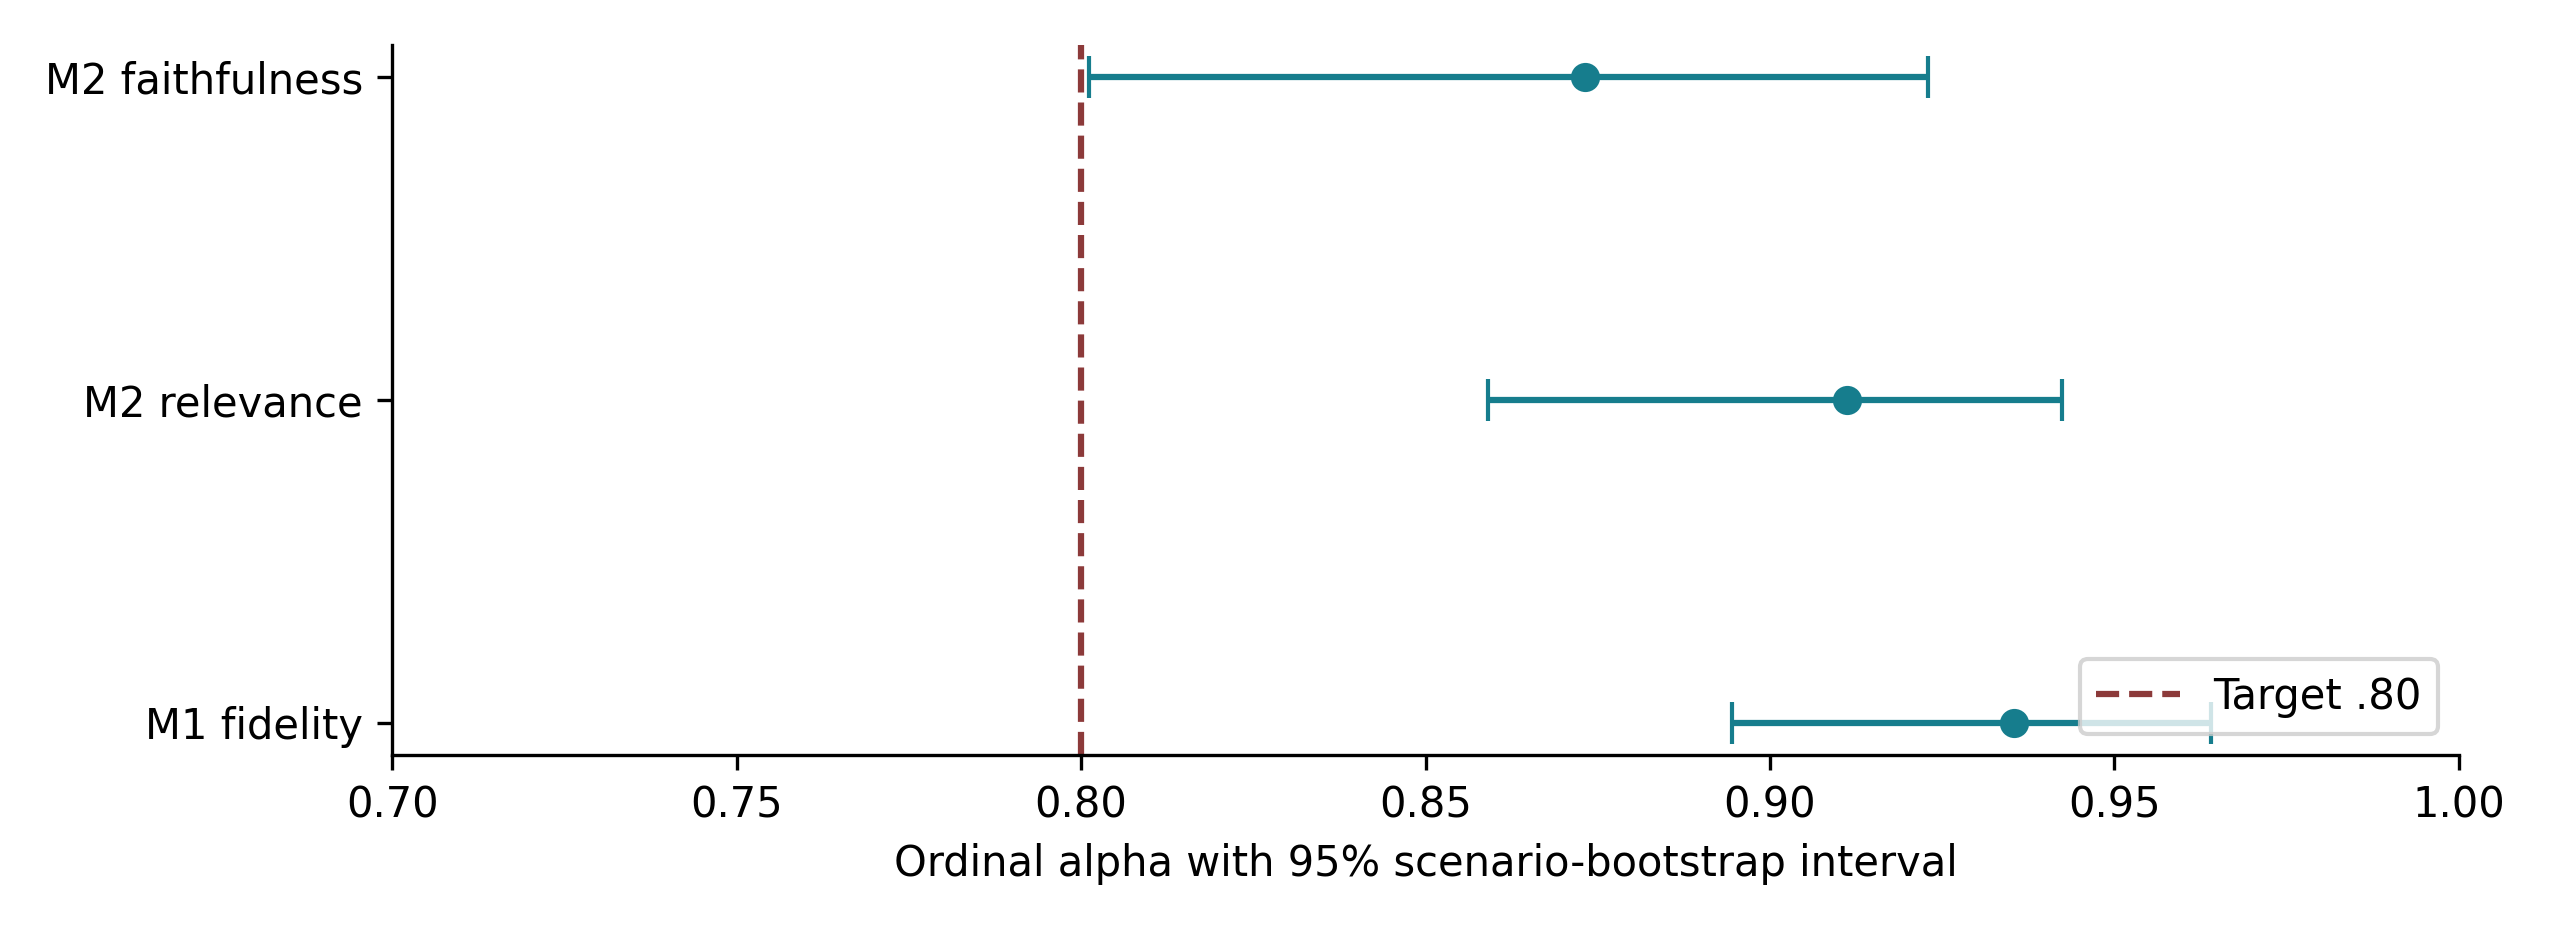
\includegraphics[width=\textwidth]{../figures/figure_4_3_agreement.png}\end{center}

Figure 4.3. Agreement point estimates and scenario-bootstrap percentile intervals. The dashed line marks the manuscript's .80 target, not a significance threshold for system superiority.


The ordinal coefficients were .9354 for normalization fidelity, .9112 for relevance and .8732 for faithfulness. All exceed the manuscript's .80 target. The estimated interval for faithfulness begins near .801, so the lower bound should not be described as comfortably above the target. Bootstrap uncertainty is conditional on the supplied ratings and sampled scenario structure. The observed experts are treated as a fixed panel; the intervals do not represent variation over all possible auditors.


High agreement indicates consistency in the ratings relative to chance disagreement. It does not mean that the systems performed well on every inquiry, that factual references were universally correct, or that collection independence has been independently verified. The implemented ordinal calculation was checked against a separate coincidence-matrix implementation on the actual data and additional test fixtures.


\section{Paired comparisons}

The exploratory comparison plan was recorded before the present computation but after ratings and prior summaries were available. It is therefore not characterized as a preregistered confirmatory analysis. Scores were averaged within each scenario/configuration across the applicable languages and the three raters. This produced 20 paired scenario units, avoiding the mistaken treatment of 780 output reviews as independent scenarios.


Exact two-sided signed-rank tests were used for B-C normalization fidelity and for B-A, C-A and B-C on each answer dimension. Zero differences were omitted from the signed-rank distribution and ties received midranks. A joint Holm correction covered the seven primary comparisons. Group-bootstrap intervals for mean differences are descriptive and not multiplicity-adjusted confidence sets. The test assumes independent scenario groups and a symmetric distribution of differences under the null; a group sign-test sensitivity analysis also showed no p-value below .05.


{\small\begin{longtable}{@{}p{0.95in}p{0.95in}p{0.95in}p{0.95in}p{0.95in}p{0.95in}@{}}\toprule

Dimension & Contrast & Mean difference & 95\% interval & Raw p & Holm p \\ \midrule\endhead

M1 fidelity & B-C & -0.0083 & [-0.1167, 0.1000] & 0.9375 & 1.0000 \\

M2 relevance & B-A & -0.0389 & [-0.2444, 0.1890] & 0.3953 & 1.0000 \\

M2 relevance & C-A & -0.0444 & [-0.2444, 0.1778] & 0.3085 & 1.0000 \\

M2 relevance & B-C & 0.0056 & [-0.0333, 0.0444] & 1.0000 & 1.0000 \\

M2 faithfulness & B-A & 0.0111 & [-0.3333, 0.3333] & 0.8485 & 1.0000 \\

M2 faithfulness & C-A & -0.0944 & [-0.4446, 0.2444] & 0.9055 & 1.0000 \\

M2 faithfulness & B-C & 0.1056 & [0.0000, 0.2222] & 0.2500 & 1.0000 \\

\bottomrule\end{longtable}}

Table 4.8. Scenario-paired system comparisons. Positive differences favor the first configuration named in each contrast. All tests use 20 scenario groups; nonzero-group counts and rank-biserial effects are supplied in paired\_comparisons.csv.


None of the seven comparisons was statistically significant after adjustment. All Holm-adjusted p-values were 1.0000. In particular, B-C faithfulness had only three nonzero scenario differences despite a positive mean difference. This small number of informative pairs limits the strength of a superiority claim. Failure to reject a difference is not evidence of equivalence; the study did not perform an equivalence test with a prespecified practical margin.


\section{Integrated discussion of the research objectives}

Objective 1 was addressed through implementation of source-linked preprocessing, dictionary-assisted normalization, chunk-level lexical/dense retrieval and local grounded generation. Intent-sensitive normalization and explicit handling of ambiguity were part of the implemented workflow. The evaluation nevertheless shows that a working architecture is not sufficient evidence that intent or factual accuracy is preserved for every question.


Objective 2 was addressed by executing A, B and C with common generation settings and preserving their outcomes. Relative to A, the hybrid pipelines showed higher descriptive Hit@3 and MRR@3 on the original complete-label subset. The close B-C retrieval measurements and the absence of a significant human normalization difference mean that the incremental contribution of query-specific dictionary injection remains unestablished in this audit. These findings should be stated without attributing the shared benefits of normalization and hybrid retrieval exclusively to the dictionary.


Objective 3 was addressed through offline RAGAS assessment and expert evaluation against the charter evidence. Expert agreement met the stated target, but relevance means around 2.3 and faithfulness means around 2.6-2.7 leave room for procedural omissions and factual imprecision. The human comparison does not demonstrate superiority of B over A or C. The automated and human results answer related but distinct questions and should not be pooled into a single effectiveness score.


Practical deployment therefore remains a separate decision. The assistant can support retrieval of charter information, but these results do not establish that it can replace official procedural guidance, issue permits, process payments or provide general legal advice. The later citizen-facing website is a separate post-study implementation with a revised response-language prompt and operational intake experiments. Its exploratory 200-question dry run is not included in the human-score tables or the frozen A/B/C results reported here. Any demonstration must identify the loaded configuration and distinguish operational fixes from the system that produced the archived study outputs.


\section{Limitations of the results}

The fixed audit subset was selected after T07 outcomes, although its ordering rule used group identifiers within categories rather than answer quality. Later retrieval-label reconciliation increased coverage and must remain separately identified. The original held-out reference answers were retained and are not universally source-certified. Ambiguous charter text, table extraction and boundary-overlapping source spans can affect what a relevance label represents.


Shared static lexical guidance in C narrows the ablation interpretation. Cross-module answer IDs share opaque suffixes for 80 normalization outputs, allowing linkage, and output similarities can also suggest system identity. Perfect blinding should not be claimed. Earlier conflicting scoring metadata was corrected on the researcher's confirmation; statistical calculations cannot resolve that history independently. No signatures, qualifications or collection timestamps are inferred from the numerical results.


The study uses a small, category-balanced human sample and three observed raters. The inferential analyses are exploratory and do not establish general population effects, equivalence or causal improvement from dictionary injection. No user-adoption, service-time, transaction-success or legal-compliance outcomes were measured. Those potential benefits remain questions for future evaluation.


\section{Evidence sources for this chapter}

The primary methodological source is 20260923.pdf, especially Chapter 1 objectives (PDF pages 7-8), pipeline and evaluation design (PDF pages 28-36), and Table 2. The two-module allocation follows CHAPTER3\_AMENDMENT.md dated 26 October 2026. Numerical sources are the final archived matched/per-query metrics, both source-span crosswalk versions, the candidate and execution manifests, and the validated human analysis results. Exact paths and hashes are recorded in source\_manifest.json. Statistical implementation references are the Fast Krippendorff project and the SciPy signed-rank documentation, as recorded in the human analysis plan.
